\clearpage % Ends the current page and causes all figures and tables to be printed

\begin{figure*}[p] % The * makes the figure span both columns, p places the figure on a float page
  \begin{center}
 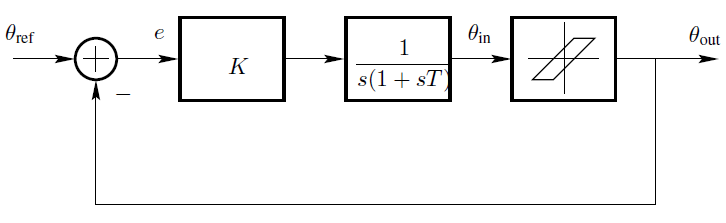
\includegraphics[width=0.8\textwidth]{images/crane.png}
  \end{center}
  \caption{Block diagram which describes the control of the angular position in a crane, obtained from ~\cite[p. 13]{Exercises:2015}. The first block represents the P controller ($K>0$), the second one the electric motor ($T>0$), and the third one the back-lash, the nonlinearity under study in this work.}
  \label{fig:crane}
\end{figure*}

\begin{figure*}[p] % The * makes the figure span both columns, p places the figure on a float page
  \begin{center}
 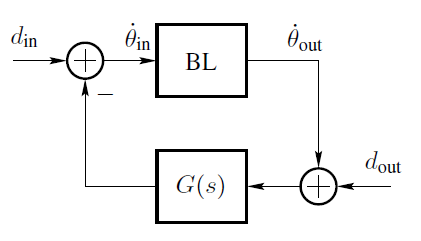
\includegraphics[width=0.5\textwidth]{images/feedback.png}
  \end{center}
  \caption{Block diagram which describes a feedback loop in which the angular-velocity back-lash model and an arbitrary linear system $G(s)$ are involved, obtained from ~\cite[p. 14]{Exercises:2015}. Signals $d_\textrm{in}$ and $d_\textrm{out}$ represents disturbances.}
  \label{fig:feedback}
\end{figure*}

\begin{figure*}[p] % The * makes the figure span both columns, p places the figure on a float page
  \begin{center}
 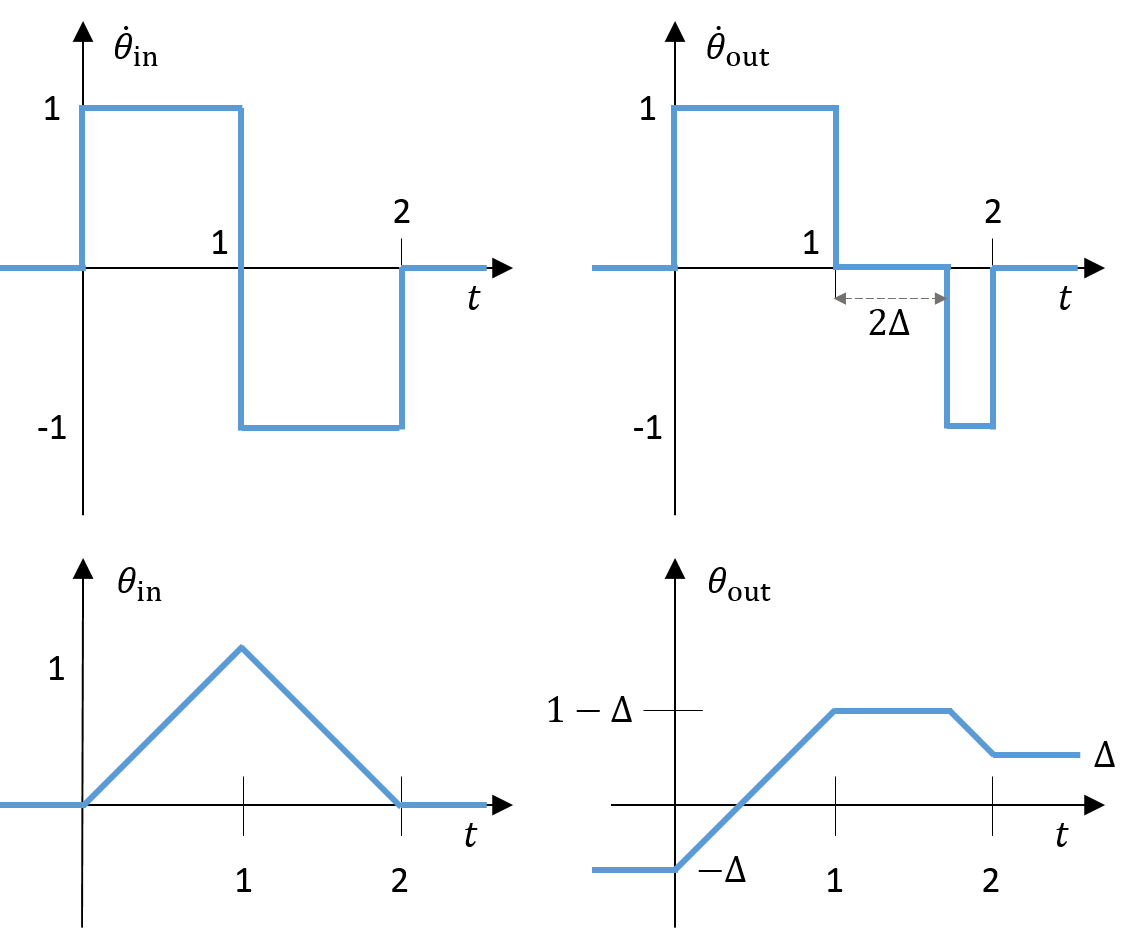
\includegraphics[width=0.7\textwidth]{images/sketch.png}
  \end{center}
  \caption{Set of sketches of $\tin$, $\tout$, $\tind$ and $\toutd$ for the angular-velocity back-lash open-loop model, when the input is the one described in equation (\ref{eq:inputBL}). Furthermore, the initial conditions are $\tin(0) = 0$ and $\tout(0) = -\Delta$.}
  \label{fig:sketch}
\end{figure*}

\begin{figure*}[p] % The * makes the figure span both columns, p places the figure on a float page
  \begin{center}
 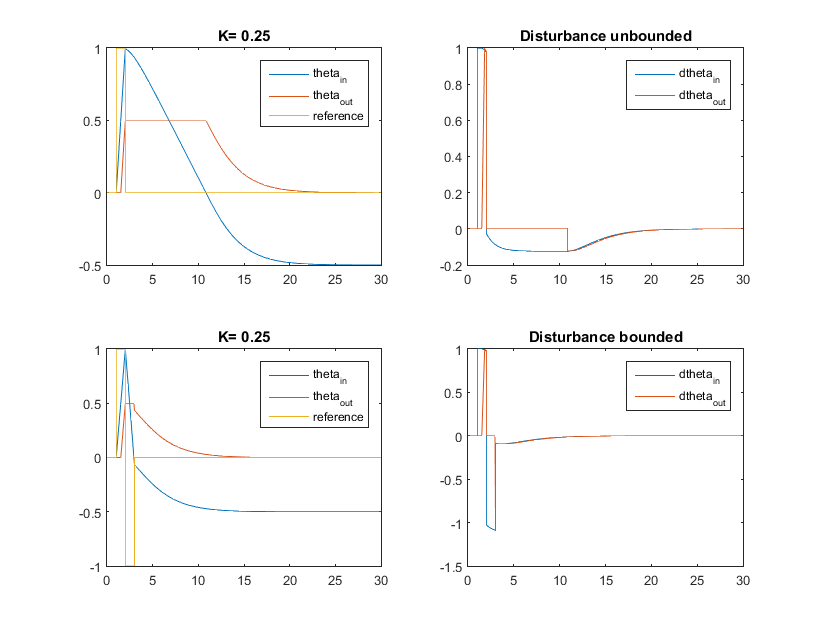
\includegraphics[width=0.75\textwidth]{images/bibo.png}
  \end{center}
  \caption{Simulated response of the system, when $K=0.25$ and for 30 seconds. The upper graphs represent the system when the disturbance is unbounded, whereas the lower graphs belongs to the bounded case.}
  \label{fig:bibo}
\end{figure*}

\begin{figure*}[p] % The * makes the figure span both columns, p places the figure on a float page
  \begin{center}
 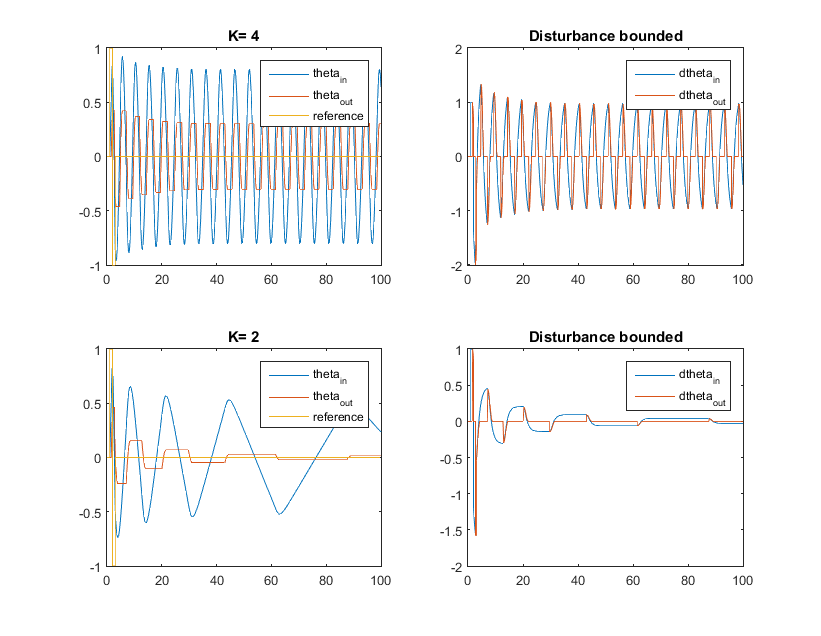
\includegraphics[width=0.75\textwidth]{images/notbibo.png}
  \end{center}
  \caption{Simulated response of the system, when the disturbance is bounded and for 100 seconds. The upper graphs represent the system when $K=4$, whereas the lower graphs belongs to the case $K=2$.}
  \label{fig:notbibo}
\end{figure*}


\begin{figure*}[p] % The * makes the figure span both columns, p places the figure on a float page
  \begin{center}
 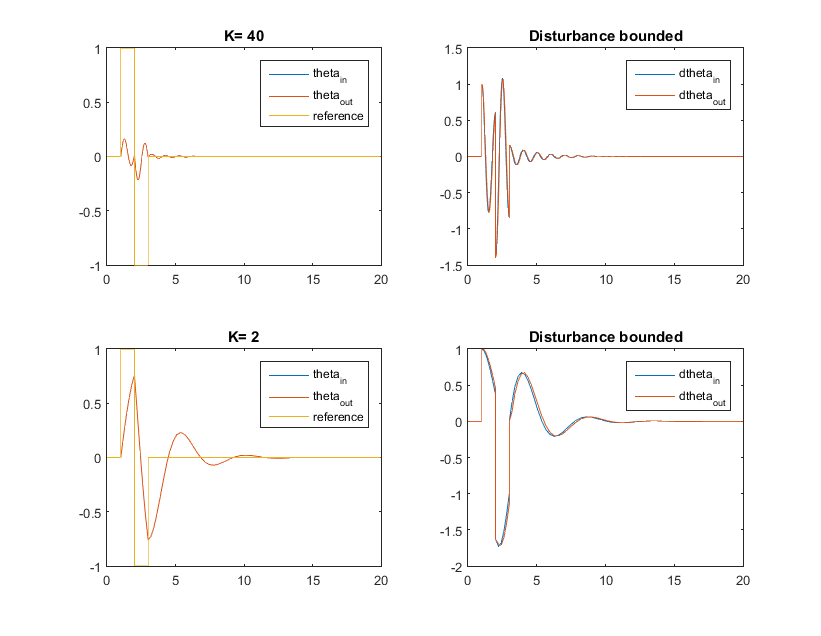
\includegraphics[width=0.75\textwidth]{images/blneglected.png}
  \end{center}
  \caption{Simulated response of the system, when the disturbance is bounded, the back-lash have been neglected and for 20 seconds. The upper graphs represent the system when $K=40$, whereas the lower graphs belongs to the case $K=2$.}
  \label{fig:blneglected}
\end{figure*}
%%%%%%%%%%%%%%%%%%%%%%%%%%%%%%%%%%%%%%%%%%%%%%%%%%%%%%%%%%%%%%%%%%%%%%%%%%%%%%%%%%%
% From example 1
%%%%%%%%%%%%%%%%%%%%%%%%%%%%%%%%%%%%%%%%%%%%%%%%%%%%%%%%%%%%%%%%%%%%%%%%%%%%%%%%%%%

% \begin{figure*}[p] % The * makes the figure span both columns, p places the figure on a float page
%   \begin{center}
%   \end{center}
%   \caption{Step response of the two systems. The figure should have a caption that briefly explains what it shows. The color, symbol and line type should be selected such that the lines can be distinguished when printed in black and white. The lines should be annotated either in the plot, in a legend, or in the caption. The axis should have a label in which the units are given. The figure should be sufficiently large, clear, easy to understand and only contain essential information.}
%   \label{fig:prestanda}
% \end{figure*}

% \begin{table*}[p] % The * makes the table span both columns, p places the table on a float page
% \caption{Jacobian matrix $A$ of the linear system $\dot{\textbf{x}} = A \textbf{x}$. The table should have a caption that briefly explains what it shows.}
% \label{tab:JacobianMatrix}
% \begin{center}
% \begin{tabular}{@{\vrule height 10.5pt depth4pt  width0pt}|c|c|c|c|}
%     \hline
%      $-2.46$ & $0$ & $-1.73$ & $0$ \\ \hline
%      $0$ & $-2.553$ & $0$ & $2.774$ \\ \hline
%      $0$ & $6.172$ & $-10$ & $7.333$ \\ \hline
%      $1.767$ & $-0.357$ & $5.714$ & $-6.074$ \\ \hline
% \end{tabular}
% \end{center}
% \end{table*}


% \begin{figure*}[p] % The * makes the figure span both columns, p places the figure on a float page
%   \begin{center}
%   \end{center}
%   \caption{Phase portrait of the system in \eqref{eqn:PPSystem}, which has a stable focus at \mbox{(0,0)} and a saddle point at \mbox{(-0.5,0)}. Both equilibriums are marked by large dots and selected trajectories are marked by solid lines. Trajectories starting within the shaded region end at the stable focus. This figure was generated in
%   Matlab (\texttt{http://www.mathworks.com}) using pplane7 (\texttt{http://math.rice.edu/\textasciitilde dfield/}).}
%   \label{fig:pplane}
% \end{figure*}